\documentclass{article}
\iffalse
This file is protected by Copyright. Please refer to the COPYRIGHT file
distributed with this source distribution.

This file is part of OpenCPI <http://www.opencpi.org>

OpenCPI is free software: you can redistribute it and/or modify it under the
terms of the GNU Lesser General Public License as published by the Free Software
Foundation, either version 3 of the License, or (at your option) any later
version.

OpenCPI is distributed in the hope that it will be useful, but WITHOUT ANY
WARRANTY; without even the implied warranty of MERCHANTABILITY or FITNESS FOR A
PARTICULAR PURPOSE. See the GNU Lesser General Public License for more details.

You should have received a copy of the GNU Lesser General Public License along
with this program. If not, see <http://www.gnu.org/licenses/>.
\fi

\author{} % Force author to be blank
%----------------------------------------------------------------------------------------
% Paper size, orientation and margins
%----------------------------------------------------------------------------------------
\usepackage{geometry}
\geometry{
	letterpaper,			% paper type
	portrait,				% text direction
	left=.75in,				% left margin
	top=.75in,				% top margin
	right=.75in,			% right margin
	bottom=.75in			% bottom margin
 }
%----------------------------------------------------------------------------------------
% Header/Footer
%----------------------------------------------------------------------------------------
\usepackage{fancyhdr} \pagestyle{fancy} % required for fancy headers
\renewcommand{\headrulewidth}{0.5pt}
\renewcommand{\footrulewidth}{0.5pt}
\rhead{\small{ANGRYVIPER Team}}
%----------------------------------------------------------------------------------------
% Appendix packages
%----------------------------------------------------------------------------------------
\usepackage[toc,page]{appendix}
%----------------------------------------------------------------------------------------
% Defined Commands & Renamed Commands
%----------------------------------------------------------------------------------------
\renewcommand{\contentsname}{Table of Contents}
\renewcommand{\listfigurename}{List of Figures}
\renewcommand{\listtablename}{List of Tables}
\newcommand{\todo}[1]{\textcolor{red}{TODO: #1}\PackageWarning{TODO:}{#1}} % To do notes
\newcommand{\code}[1]{\texttt{#1}} % For inline code snippet or command line
%----------------------------------------------------------------------------------------
% Various packages
%----------------------------------------------------------------------------------------
\usepackage{hyperref} % for linking urls and lists
\usepackage{graphicx} % for including pictures by file
\usepackage{listings} % for coding language styles
\usepackage{rotating} % for sideways table
\usepackage{pifont}   % for sideways table
\usepackage{pdflscape} % for landscape view
%----------------------------------------------------------------------------------------
% Table packages
%----------------------------------------------------------------------------------------
\usepackage{tabularx} % c=center,l=left,r=right,X=fill
\usepackage{float}
\floatstyle{plaintop}
\usepackage[tableposition=top]{caption}
\newcolumntype{P}[1]{>{\centering\arraybackslash}p{#1}}
\newcolumntype{M}[1]{>{\centering\arraybackslash}m{#1}}
%----------------------------------------------------------------------------------------
% Block Diagram / FSM Drawings
%----------------------------------------------------------------------------------------
\usepackage{tikz}
\usetikzlibrary{shapes,arrows,fit,positioning}
\usetikzlibrary{automata} % used for the fsm
%----------------------------------------------------------------------------------------
% Colors Used
%----------------------------------------------------------------------------------------
\usepackage{colortbl}
\definecolor{blue}{rgb}{.7,.8,.9}
\definecolor{ceruleanblue}{rgb}{0.16, 0.32, 0.75}
\definecolor{drkgreen}{rgb}{0,0.6,0}
\definecolor{deepmagenta}{rgb}{0.8, 0.0, 0.8}
\definecolor{cyan}{rgb}{0.0,0.6,0.6}
\definecolor{maroon}{rgb}{0.5,0,0}
%----------------------------------------------------------------------------------------
% Update the docTitle and docVersion per document
%----------------------------------------------------------------------------------------
\def\docTitle{Component Data Sheet}
\def\docVersion{1.1}
%----------------------------------------------------------------------------------------
\date{Version \docVersion} % Force date to be blank and override date with version
\title{\docTitle}
\lhead{\small{\docTitle}}

\def\comp{complex\_mixer}
\def\Comp{Complex Mixer}
\graphicspath{ {figures/} }

\begin{document}

\section*{Summary - \Comp}
\begin{tabular}{|c|M{13.5cm}|}
	\hline
	\rowcolor{blue}
	                  &                                                    \\
	\hline
	Name              & \comp                                              \\
	\hline
	Worker Type       & Application                                        \\
	\hline
	Version           & v1.2                                              \\
	\hline
	Release Date      & August 2017                                        \\
	\hline
	Component Library & ocpi.training.components                                  \\
	\hline
	Workers           & \comp.hdl \comp.rcc                               \\
	\hline
	Tested Platforms  & c7-x86\_64, linux-x13\_3-arm, xsim, Matchstiq-Z1(PL)(Vivado 2017.1)\\
	\hline
\end{tabular}

\section*{Functionality}
\begin{flushleft}
	The Complex Mixer consists of a Numerically Controlled Oscillator (NCO) and a complex multiplier. Complex IQ data is received on the input port and is multiplied with the output of the NCO and put on the output port.
\end{flushleft}

\section*{Worker Implementation Details}
\subsection*{\comp.hdl}
\begin{flushleft}
	Figure \ref{fig:complex_mixer} diagrams the complex mixer.\medskip

	\begin{figure}[h]
		\centering\captionsetup{type=figure}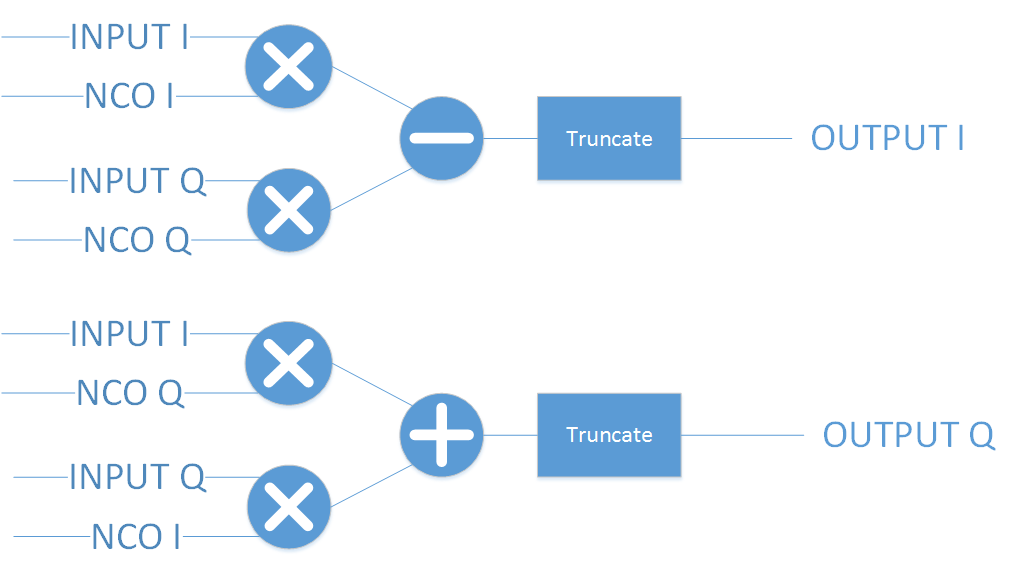
\includegraphics[scale=0.4]{complex_mixer_block_diagram}
		\captionof{figure}{Complex Mixer Functional Diagram}
		\label{fig:complex_mixer}
	\end{figure}

	The control properties for all implementations provide the ability to \textit{enable}(or bypass) the worker and set the tune frequency via \textit{phs\_inc}.\medskip

	The HDL worker leverages Xilinx Vivado cores to implement the NCO (DDS Compiler v6.0.13) and complex multiply (Complex Multiplier v6.0.12) functions. The Vivado IP Catalog tool was used to generate both cores. For both cores, their respective default configuration settings were chosen with the following exceptions:

	\begin{itemize}
		\item DDS Compiler 6.0.13 (dds\_compiler.xci)
			\subitem Parameter Selection = Hardware Parameters
			\subitem Output Width = 16
			\subitem Phase Increment Programmabililty = Streaming
			\subitem Optional Pins: Has Phase Out is unchecked and ARESETn checked
		\item Complex Multiplier v6.0.12 (complex\_multiplier.xci)
			\subitem Control Signals: ACLKEN and ARESETn checked
	\end{itemize}

	The dds\_compliler v6.0.13 implements a phase generator and sin/cos look-up tables (LUT), and has a latency of 7.  The complex\_multiplier v6.0.12 uses 3 DSP48E1s and has a latency of 6.\medskip

	In conjunction with the \textit{enable}(or bypass) control property, the HDL worker provides the ability to select different (\textit{data\_select}) data to output in bypass mode: input or output of the NCO.\medskip
\end{flushleft}
\subsection*{\comp.rcc}
\begin{flushleft}
	The RCC worker leverages liquid-dsp v1.2 and its \textit{nco} class to generate the internal NCO used in the algorithm. More information on this liquid-dsp module can be seen in the online documentation: \href{http://liquidsdr.org/doc/nco/}{liquid-dsp}.  \\
	In the RCC version of this component the samples are converted from fixed point to floating point numbers in order to do that math on a GPP. This conversion introduces a small amount of error in the output data and should be accounted for when it is used in an application.  The conversion equations are as follows:

	\begin{equation} \label{eq:iq_float}
  		iq\_float = \frac{iq\_fixed}{2^{15} -1}
	\end{equation}

    \begin{equation} \label{eq:iq_fixed}
  		iq\_fixed = {iq\_float}*(2^{15} -1)
	\end{equation}

	In the RCC worker a conversion needs to be done for the phase increment to adhere to the way the HDL phase increment is implemented.  The conversion was done in the RCC version of this component because the division operation is very resource intensive in HDL.  The conversion from the component property to the liquid-dsp interface input property is as follows:
	\begin{equation} \label{eq:rcc_phase_inc}
  		liquid\_phs\_inc = phs\_inc*\frac{2\pi}{0x7FFF*2}
	\end{equation}
\end{flushleft}

\section*{Theory}
\begin{flushleft}
	The Complex Mixer worker inputs complex signed samples and performs a complex multiply with a digital sine wave produced by an numerically controlled oscillator (NCO). The resulting output data is a frequency shifted version of the input data.\medskip

	The magnitude of the frequency shift is determined by the output frequency of the NCO, which can be calculated with the following equation:

	\begin{equation} \label{eq:nco_output_freq}
		nco\_output\_freq = sample\_freq*\frac{phs\_inc}{2^{phs\_acc\_width}}
	\end{equation}

	In this component, \verb+phs_inc+ is runtime configurable and has a data type of 16 bit signed short. \verb+phs_acc_width+ is fixed at 16. The input clock frequency is the sample rate of the samples. The amplitude of the NCO's sine wave is fixed at the full range of a signed 16 bit value.
\end{flushleft}

\section*{Block Diagrams}
\subsection*{Top level}
	\begin{center}
		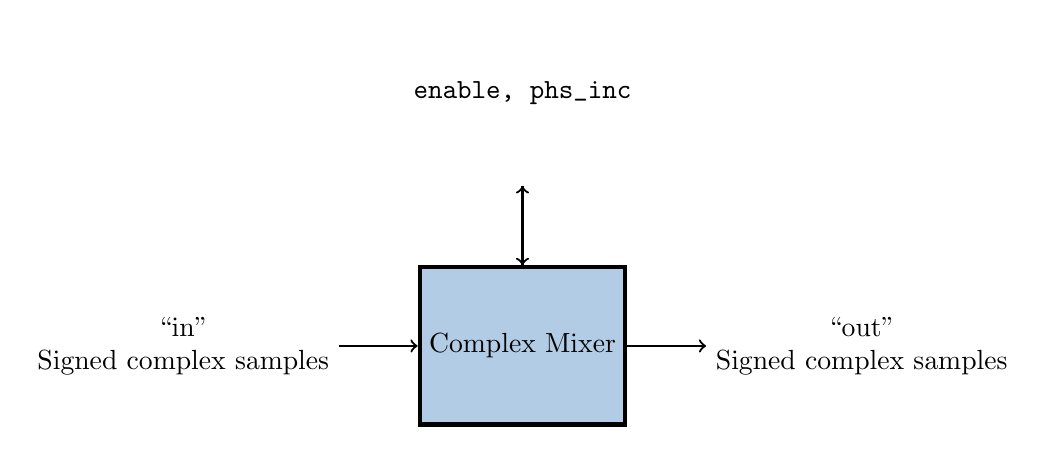
\begin{tikzpicture}[% List of styles applied to all, to override specify on a case-by-case
				every node/.style={
					align=center,  		% use this so that the "\\" for line break works
					minimum size=2cm	% creates space above and below text in rectangle
				},
				every edge/.style={draw,thick}
			]
			\node[rectangle,ultra thick,draw=black,fill=blue](R2){\Comp};
			\node[rectangle,draw=white,fill=white](R3)[left= of R2]{``in" \\ Signed complex samples};
			\node[rectangle,draw=white,fill=white](R4)[right= of R2]{``out" \\ Signed complex samples};
			\node[rectangle,draw=white,fill=white](R5)[above= of R2]{\verb+enable, phs_inc+\\};
			\path[->]
			(R3)edge []	node [] {} (R2)
			(R2)edge []	node [] {} (R4)
			(R2)edge []	node [] {} (R5)
			(R5)edge []	node [] {} (R2)
			;
		\end{tikzpicture}
	\end{center}
	\captionof{figure}{Complex Mixer Top Level Block Diagram}
	\label{fig:block_diagram}

\newpage
\subsection*{State Machine}
	Not Applicable

\section*{Source Dependencies}
\subsection*{\comp.rcc}
   \begin{itemize}
      \item Liquid DSP (provided as \path{av-prereq-liquid-*.rpm})
   \end{itemize}
\subsection*{\comp.hdl}
	\begin{itemize}
		\item training\_project/components/complex\_mixer.hdl/complex\_mixer.vhd
		\item
training\_project/components/complex\_mixer.hdl/vivado\_ip/complex\_multiplier\_stub.vhd
		\item
training\_project/components/complex\_mixer.hdl/vivado\_ip/complex\_multiplier\_sim\_net.vhd
		\item
training\_project/components/complex\_mixer.hdl/vivado\_ip/complex\_multiplier.vho
		\item
training\_project/components/complex\_mixer.hdl/vivado\_ip/complex\_multiplier.xci
		\item
training\_project/components/complex\_mixer.hdl/vivado\_ip/complex\_multiplier.edf
		\item training\_project/components/complex\_mixer.hdl/vivado\_ip/dds\_compiler\_stub.vhd
		\item training\_project/components/complex\_mixer.hdl/vivado\_ip/dds\_compiler\_sim\_net.vhd
		\item
training\_project/components/complex\_mixer.hdl/vivado\_ip/dds\_compiler.vho
		\item
training\_project/components/complex\_mixer.hdl/vivado\_ip/dds\_compiler.xci
		\item
training\_project/components/complex\_mixer.hdl/vivado\_ip/dds\_compiler.edf
	\end{itemize}

\begin{landscape}
	\section*{Component Spec Properties}
	\begin{scriptsize}
		\begin{tabular}{|p{3cm}|p{1.5cm}|c|c|c|p{1.5cm}|p{1cm}|p{7cm}|}
			\hline
			\rowcolor{blue}
			Name               & Type   & SequenceLength & ArrayDimensions & Accessibility      & Valid Range & Default & Usage                                                                         \\
			\hline
			\verb+enable+      & Bool   & -              & -               & Writable & Standard    & true    & Enable(true) or bypass(false) mixer                                           \\
			\hline
			\verb+phs_inc+     & Short  & -              & -               & Writable & *           & -8192   & Phase increment of NCO \scriptsize\begin{verbatim} * -2^(NCO_DATA_WIDTH_p-1)
			to +2^(NCO_DATA_WIDTH_p-1)-1\end{verbatim}\\
			\hline

		\end{tabular}
	\end{scriptsize}

	\section*{Worker Properties}
	\subsection*{\comp.hdl}
	\begin{scriptsize}
		\begin{tabular}{|p{1.5cm}|p{2.5cm}|p{1cm}|c|c|c|p{2cm}|p{1cm}|p{5cm}|}
			\hline
			\rowcolor{blue}
			Type     & Name                      & Type  & SequenceLength & ArrayDimensions & Accessibility       & Valid Range & Default & Usage                                      \\
			\hline
			Property & \verb+data_select+     & Bool  & -              & -               & Writable & Standard    & false    & In Bypass Mode: selects data to output: 0=input data, 1=output of NCO   \\
			\hline
		\end{tabular}
	\end{scriptsize}

	\section*{Component Ports}
	\begin{scriptsize}
		\begin{tabular}{|M{2cm}|M{1.5cm}|M{4cm}|c|c|M{9cm}|}
			\hline
			\rowcolor{blue}
			Name & Producer & Protocol           & Optional & Advanced & Usage                  \\
			\hline
			in   & false    & iqstream\_protocol & false    & -        & Signed complex samples \\
			\hline
			out  & true     & iqstream\_protocol & false    & -        & Signed complex samples \\
			\hline
		\end{tabular}
	\end{scriptsize}

	\section*{Worker Interfaces}
	\subsection*{\comp.hdl}
	\begin{scriptsize}
		\begin{tabular}{|M{2cm}|M{1.5cm}|c|c|M{12cm}|}
			\hline
			\rowcolor{blue}
			Type            & Name & DataWidth & Advanced                & Usage                  \\
			\hline
			StreamInterface & in   & 32        & - & Signed Complex Samples \\
			\hline
			\rowcolor{blue}
			Type            & Name & DataWidth & Advanced                & Usage                  \\
			\hline
			StreamInterface & out  & 32        & - & Signed Complex Samples \\
			\hline
		\end{tabular}
	\end{scriptsize}
\end{landscape}

\section*{Control Timing and Signals}
\begin{flushleft}
	The Complex Mixer HDL worker uses the clock from the Control Plane and standard Control Plane signals.\medskip

	There is a startup delay for this worker. Once the input is ready and valid and the output is ready, there is a 6 clock cycle start delay (pipeline delay of complex multiplier). After this startup delay, valid output data is given 6 clock cycles after input data is taken.

	\begin{tabular}{|M{4.5cm}|M{1cm}|M{1cm}|M{1.5cm}|M{2cm}|M{1cm}|M{1cm}|M{2.5cm}|}
		\hline
		\rowcolor{blue}
		Latency         \\
		\hline
		6 clock cycles  \\
		\hline
	\end{tabular}
\end{flushleft}

\section*{Performance and Resource Utilization}
	\subsubsection*{RCC}
	    Needs to be tested to populate this section.
	\subsubsection*{HDL}
		\begin{scriptsize}
		\begin{tabular}{|c|c|c|c|c|c|c|c|}
			\hline
			\rowcolor{blue}
			Device & Registers & LUTs & Fmax & Memory/Special Functions & Design Suite\\
			\hline
            Zynq XC7Z020-1-CLG484    & 450    & 252 & 307.882 MHz & DSP48E1 = 3 & Vivado 2017.1\\
			\hline
		\end{tabular}
		\end{scriptsize}

\section*{Test and Verification}
\begin{flushleft}
	Test cases are derived from the number of properties, and their respective values, as listed in the complex\_mixer-test.xml. Specifically, the \comp.rcc and \comp.hdl implementations tested, as follows:

	\begin{itemize}
		\item[1)] Bypass (RCC \& HDL): The input data is forwarded to the output port. For 				verification of this case, the output file is byte-wise compared to the input file.
		\item[2)] Normal mode (RCC \& HDL): The NCO is configured to tune the input signal to 		baseband. For verification, an FFT of the output data is performed and the max value 			of the FFT is checked to be at DC (0 Hz).
		%	\item[3)] Bypass mode/data_select=1 : NCO output is captured (HDL)
	\end{itemize}

For all cases, the input file contains a tone of 12.5 Hz sampled at 100 Hz and an amplitude of 32767.
\end{flushleft}

\end{document}
